\begin{savequote}[75mm]
In that sense, this new knowledge has all to do with honor and country but it has nothing to do directly with defending our country except to help make it worth defending. 
\qauthor{Robert R. Wilson during the Congressional Testimony on building Fermilab's first accelerator}
\end{savequote}


\chapter{The LHCb Experiment and its Upgrade}

This chapter presents a detailed description of the LHCb experiment. Before I move to the explanation of the technical details of the LHCb detector, I am going to outline its background. 
This section starts by presenting the CERN (The European Organization for Nuclear Research) . Then, I'll try to give you a basic understanding of how the LHC ( \textsc{Large Hadron Collider}, the most powerful particle accelerator, works. On the next couple of pages, I will explain the Standard Model and the Physics motivation to construct the LHCb detector. The final part of this chapter presents a technical aspect of the LHCb detector. I cover the current architecture as well as the plans and motivation for the future upgrade. 
\section{CERN}
The European Organization for Nuclear Research CERN is the world largest scientific organization in the field of High Energy Physics. It was established in 1954 by twelve western European countries to create one of the very first European joint venture. Currently, the CERN associate 22 members state including Poland. The Institution is based on the Swiss-France border very close to Geneva. The main focus of the CERN is to design and construct instruments to study the fundamental building of matter and its interactions.  

\begingroup
    \expandafter\patchcmd\csname Gin@ii\endcsname   % needed etoolbox
      {\setkeys {Gin}{#1}}
      {\setkeys {Gin}
          {width=\linewidth,                     % standard graphicx settings
           valign=c, margin=-3pt 6pt 0pt 6pt,#1}     % settings from adjustbox
      }
      {}{}

\section{Large Hadron Collider}
The Large Hadron Collider (LHC) is the word largest circular particle accelerator. It is installed in the 26.7 km long tunnel that was constructed for the previous experiment Large Electron Positon Collider (LEP) [cite]. The tunnel is situated about 100 m below the ground. 
The LHC is designed to accelerate the protons and heavy ions. At the nominal performance, the LHC delivers the two protons beams of energy 6.5 TeV.  This corresponds to the center-of-mass collision energy of 13 TeV. 
To achieve this performance the particle acceleration is done by a series of accelerators. Each of it progressively boosts the energy of the beam. Figure \ref{fig:LHC} shows the LHC accelerator complex. 

\begin{figure}
\centering
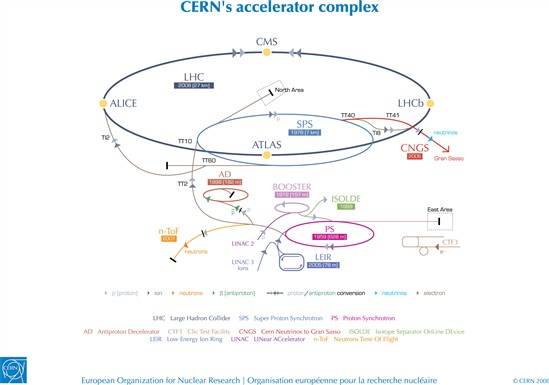
\includegraphics{figures/LHC.jpg}
\caption{The LHC accelerator complex showing all accelerator facilities and the four main experiments.
\label{fig:LHC}}
\end{figure}

The entire boosting process starts from the small red bottle full of hydrogen. It is shown in figure \ref{fig:Bottle}. This bottle is the only and sufficient proton source for entire, huge LHC acceleration system. This shows, how sophisticated and resource efficient LHC is. Then, the hydrogen atoms are ionized by the external electric field to yield the protons. These particles are injected into the Liniac2, the first linear accelerator in the chain, to boost its energy to the 50 MeV. After that, the beam is inserted into the Proton Synchrotron Booster followed by the Proton Synchrotron (PS), which pushes the beam to the energy of 25 GeV. The next step in the acceleration sequence is performed by the Super Proton Synchrotron (SPS). It accelerates the beam to the energy of 450 GeV. 

The protons are finally injected into two beam pipes of the LHC. The beam in one pipe circulates clockwise while the beam in the second pipe circulates anticlockwise. It takes 4 minutes and 20 seconds to fill each LHC ring, and 20 minutes for the protons to reach their maximum energy of 6.5 TeV. The two beams interact inside four detectors – ALICE, ATLAS, CMS, and LHCb.

\begin{figure}
\centering
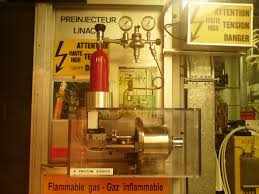
\includegraphics[scale=0.6]{figures/Bottle.jpg}
\caption{The LHC proton source 
\label{fig:Bottle}}
\end{figure}



\section{LHCb detrctor}

The heart of the LHCb experiment is its detector. It was built to produce proton-proton collision at center-of-mass energy of 14 TeV. It is located in the cavern that previously was used to host the LEP's experiment Delphi. The most unique feature of the LHCb detector is its shape. It is significantly different from the shape of other general purpose detectors like Atlas or CMS, which look like a multi-layer barrels around the collision point. For the comparison, the LHCb is a forward single-arm spectrometer. The choice of such layout was motivated by the LHCb physics program, in particular the angular distribution of the $\overline{b}b$ pairs production, which are concentrated around the forward and backward cones, see figure \ref{fig:bb}.

LHCb geometrical coverage corresponds to only 4\% of whole solid angle, but it covers the region where probability of finding the  $\overline{b}b$ pairs is 24\% and 27\% for a single $b$ or $\overline{b}$ hadrons. 


\begin{figure}[h]
 \begin{center}
  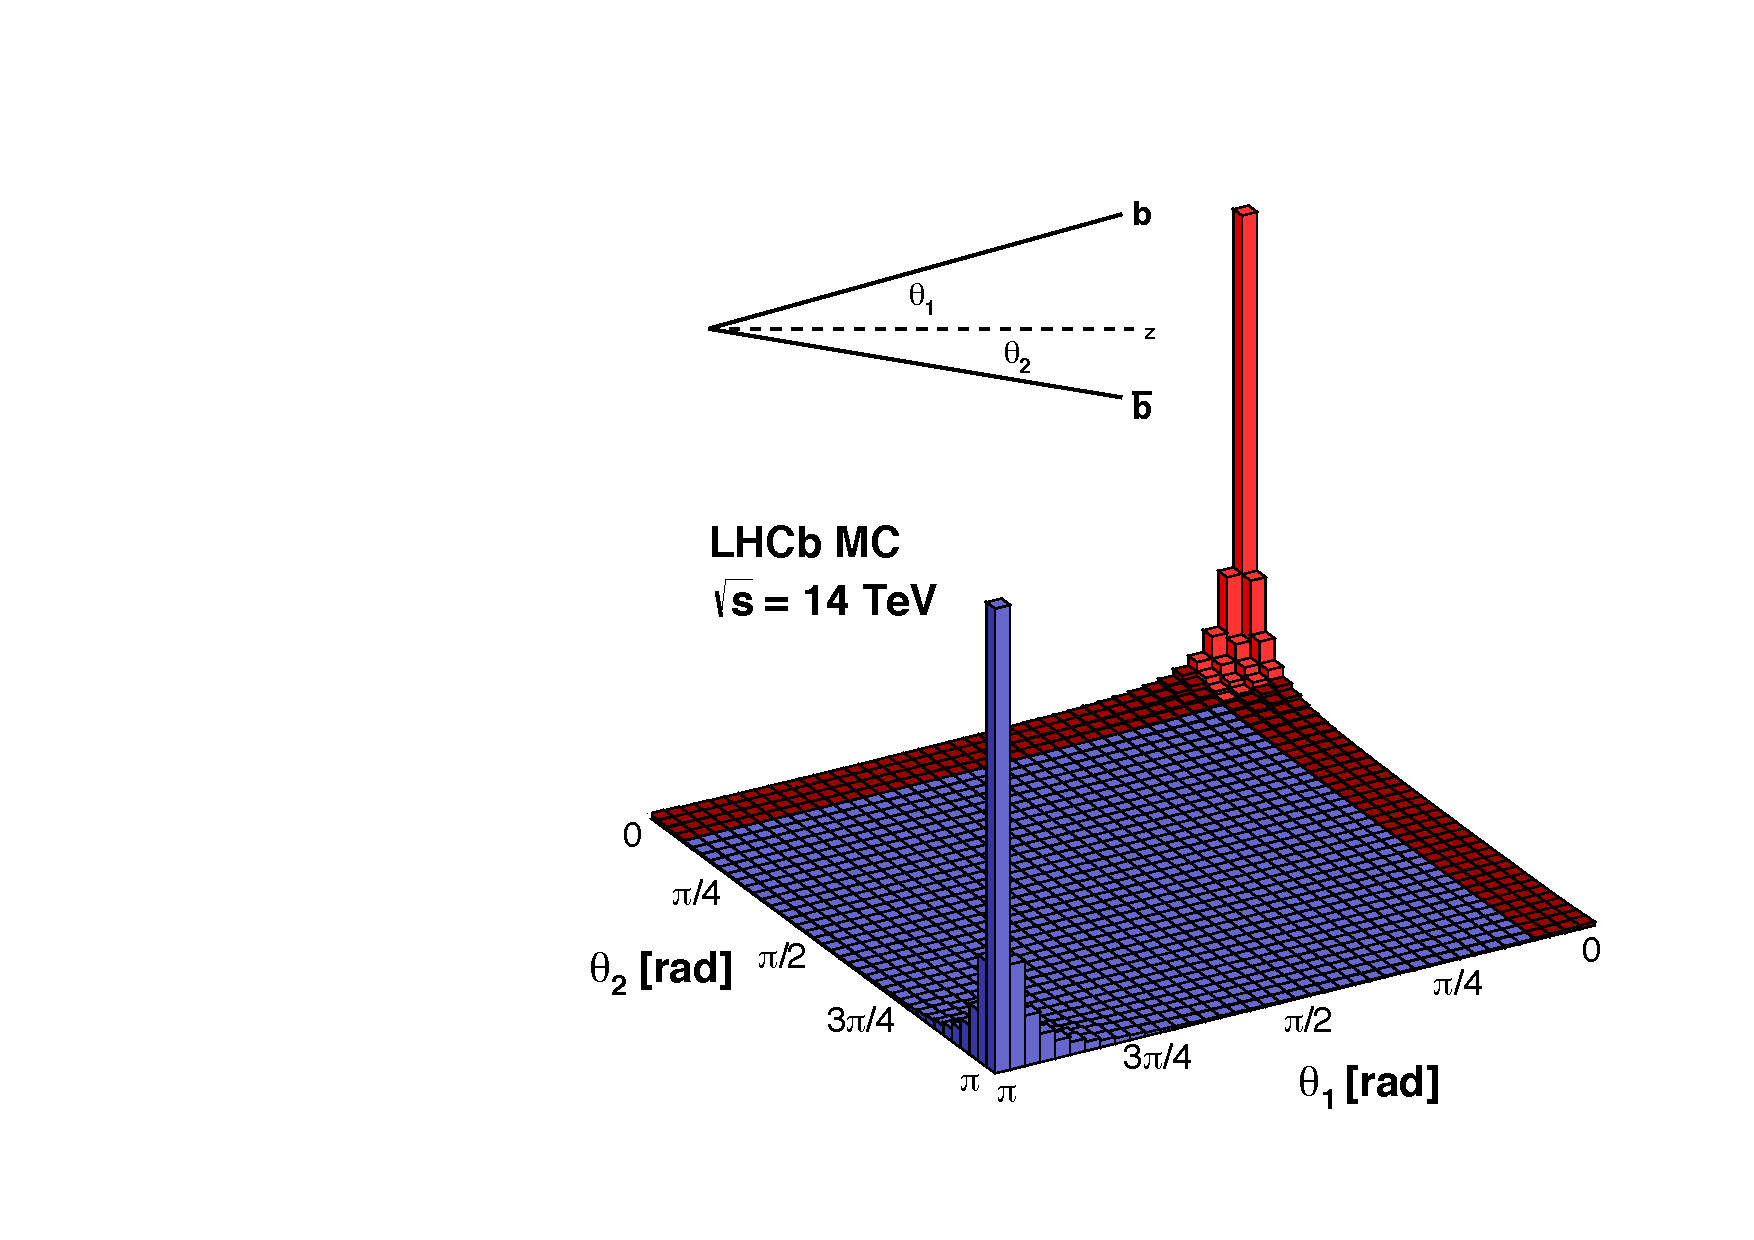
\includegraphics[width=0.40\linewidth]{figures/bb_1.pdf}
   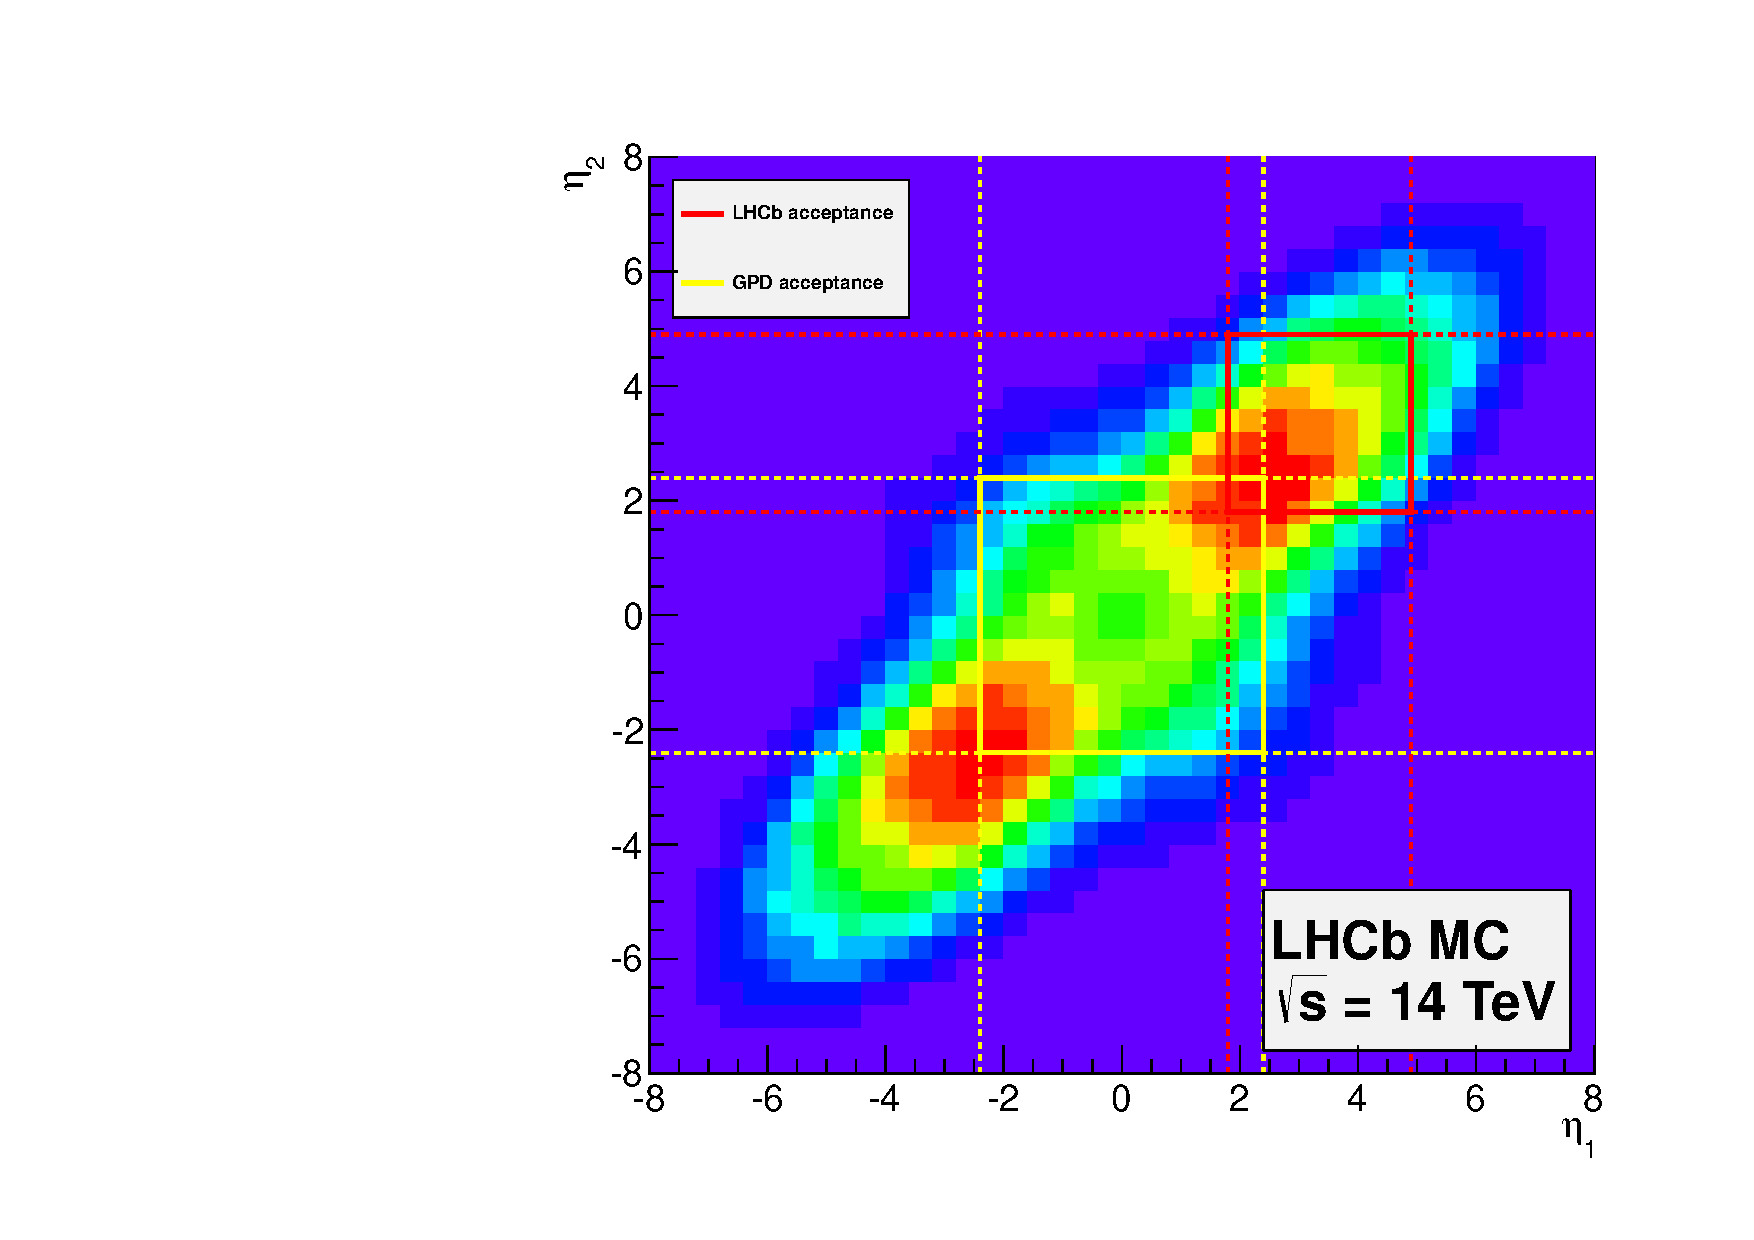
\includegraphics[width=0.35\linewidth,angle=270]{figures/bb_2.pdf}
   \caption{Production of  $\overline{b}b$ quarks at LHC at 14 TeV. Left plot present the production of the $\overline{b}b$ quarks as a function of polar angle $\theta$. Right plot show the same distribution as a function of a rapidity of each quark. The pseudorapidity region inside a yellow square corresponds to the acceptance region of the Atlas and CMS detector, while the red box highlight acceptance region of LHCb. Figure taken from \cite{bbangles}. 
     \label{fig:bb}}
 \end{center}
\end{figure}

The LHCb, like all of the currently operating High Energy Physics experiments, consist of a number of sub-detectors, each of it was carefully designed to provide an information that allows to discover, previously unseen physics phenomena. In order to correctly identify and reconstruct the decays and theirs kinematical properties LHCb detector needs to provide excellent vertex determination, momentum resolution and particle identification. The following section is dedicated to describe each of the sub-system. 

\subsection{LCHb tracking subsystem}
\label{sec:lhcb_tracking_subsystem}
The tracking system was designed to reconstruct the trajectory of charged particles by combining information from a set of tracking stations. The reconstructed track information is used to estimate the momentum of the charged particles. This estimation is possible due to installation the Magnet, which creates a magnetic field used to bend a particle trajectory. The LHCb tracking system is composed of the Vertex Locator (VELO), the Tracker Turicensis (TT), and the three tracking stations T1,T2 and T3, see \ref{fig:LHCBlayout}.  The brief description of each tracking sub-detectors is a topic of this subsection. 

\subsubsection{Velo}

The Vertex Locator is a silicon strip detector that is located close to the proton-proton collision point and it is dedicated to provide precise measurements of the position of the primary and secondary vertices \footnote{The secondary vertex is a point of decay of short lived particles, which was created in the primary interaction. }, which are essential to identify $b$ and $c$ hadrons, which typically traverse about 1 cm at LHCb.  
In fact, VELO active area is just about 8 mm away from the beam line, which is the word record. Additionally, the Velo allows precisely measure the Impact Parameter of charged particles trajectories. Impact Parameter is a transverse distance of closest approach between a particle trajectory and a vertex, most commonly the primary proton-proton interaction vertex. The impact parameter is widely used in many LHCb data analysis to make a selection that significantly reduce the contamination from the light-quark backgrounds.  


The Velo is composed by 21 silicon tracking stations positioned along the beam axis ($z$). Each of the tracking station is divided into two movable halves, called modules, consorting of two silicon microstrip sensors. Figure \ref{fig:veloLayout} presents the layout of the Velo detector. To minimize the amount of the material with which particle traversing detector can interact, all Velo sensors operate in the vacuum. The Velo vacuum is separated from the beam vacuum by a thin aluminium layer called RF foil.   


\begin{figure}[h]
\centering
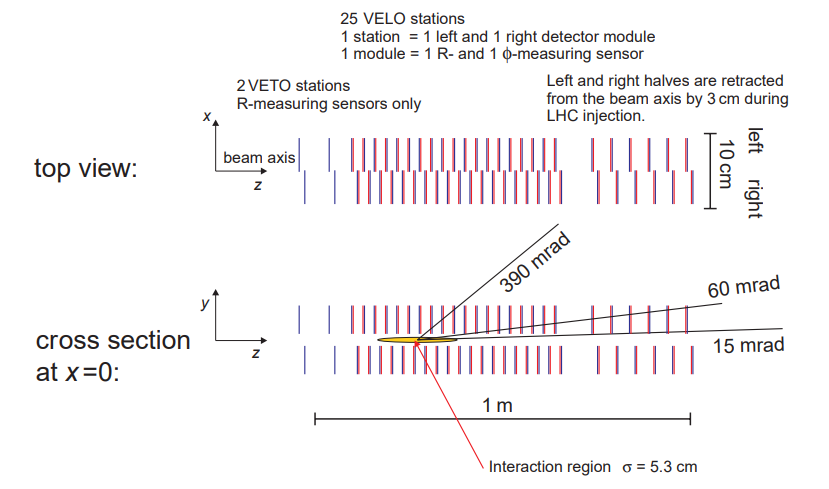
\includegraphics{figures/VeloLayout.png}
\caption{Layout of the Velo. The top figure presents the Velo setup seen from the top, indicating the overlap between the left and right detector's halves. The bottom figure is a cross section of the Velo at $x=0$. The three black lines indicate the maximum and minimum angular coverage of the Velo and the average angle of the tracks. Figure taken from \cite{VeloTDR} 
\label{fig:veloLayout}}
\end{figure}


The first type of the Velo sensor is called $R$, and it is dedicated to measure $r$-coordinate. Its pitch \footnote{Pitch is a distance between the centres of two adjacent strips} increases linearly from $38\mu m$ at the innermost region to $102 \mu m$. The  $\varphi$ sensor are further divided into two regions, inner and outer, with different pitches in order to cope with high occupancies. The geometry of the Velo sensors is presented in figure \ref{fig:velo}. Both $R$ and $\varphi$ sensors has thickness of $300 \mu m$. The Velo sensors and readout electronic are cooled by the evaporated $CO_2$ system. This system cools down the sensors to the temperature of $-8^\circ$C during data taking.  


\begin{figure}[h]
 \begin{center}
  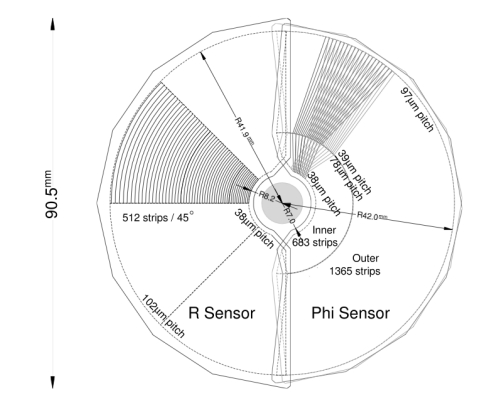
\includegraphics[width=0.49\linewidth]{figures/VeloGeometry.PNG}
   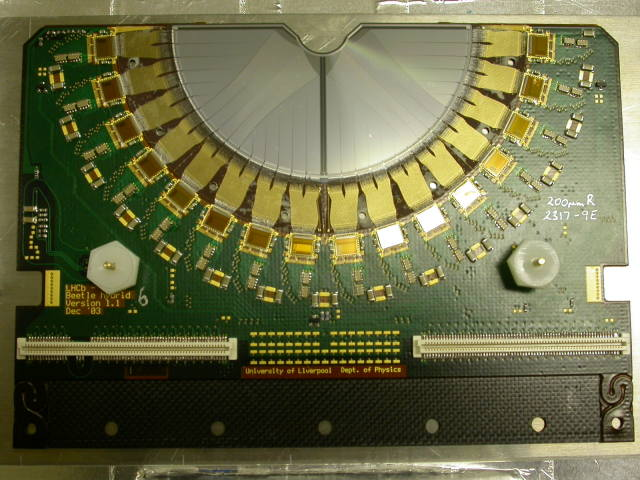
\includegraphics[width=0.49\linewidth]{figures/Velo_photo.jpg}
   \caption{Geometry of the Velo $R$ and  $\varphi$ sensors, with only a small portion of strips visible for clarity (left). The photo of the Velo module with 16 readout Beetle chips (right). Figures taken from\cite{lhcb}.  
     \label{fig:velo}}
 \end{center}
\end{figure}

The readout of the data is performed by the Beetle front-end ASIC\footnote{ASIC stands from Application-specific integrated circuit}\cite{beetle}. These chips are placed on the outer edge of the sensor, see figure \ref{fig:velo}. The Beetle chip integrates 128 channels with low-noise charge-sensitive preamplifiers and shapers, an analogue pipelined memory and a multiplexer.


The Velo detector delivers primary vertex measurements characterized by the excellent spatial resolution of about $13 \mu m $ in the transverse plane and nearly $70 \mu m $ along the $z$ axis. The dependence of the primary vertex resolution versus number of tracks obtained using 2012 calibration data is shown in figure \ref{fig:veloPerformance}. The resolution of the Impact Parameter depends on  multiple scattering, primary vertex resolution and single-hit resolution can be expressed as a function of transverse momentum $p_t$ \cite{veloPerformance}: 

\begin{equation}
    \sigma_{IP} = \left( 11.5  + \frac{24.5}{p_t[GeV/c^2]} \right)
\end{equation}



\begin{figure}[h]
\centering
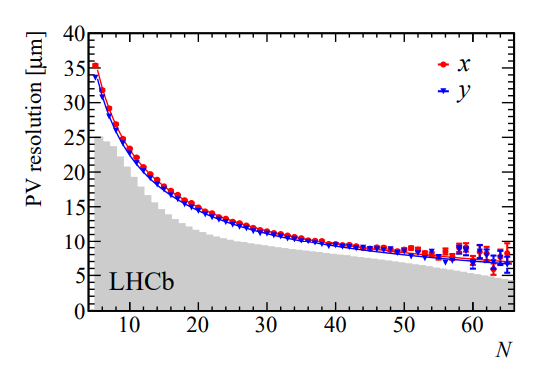
\includegraphics{figures/VeloResolution.PNG}
\caption{Primary vertex resolution as a function of a track multiplicity. The blue curve corresponds to $y$ coordinate of the Primary Vertex, and the red one to the $y$ coordinate. The gray histogram presents the number of tracks per reconstructed primary vertex. Presented results were obtained from 2012 calibration data with only one reconstructed primary vertex in the event. Figure taken from \cite{veloPerformance} 
\label{fig:veloPerformance}}
\end{figure}

\subsubsection{Silicon Tracker}

Silicon Tracker is a project that consists of two detectors based on similar technology and whose data is read by the same readout system. The first component of this project is called TT and it is based upstream of the magnet, while the Inner Tracker (IT) is an inner region of three tracking stations (T1, T2, T3 see figure \ref{fig:LHCBlayout}) located downstream to the magnet.

The TT goal is to reconstruct low-momentum tracks that are outside of the detector acceptance and tracks that come from the daughters of long-lived particles, which decay outside of the Velo. The IT reconstruct tracks with momentum larger than $1.5 GeV/c$ situated near the beam axis and passed through the magnetic field, covering approximately $2\%$ of the detector acceptance which corresponds to $20\%$ of all tracks that pass through T stations. On the other hand, TT is designed to cover the full LHCb acceptance region.  

Each Silicon Tracker station is composed of four planes, by convention denoted as $(X, U, V, X)$, where $X$ is a vertically oriented plane,  $U$ and $V$  represent planes that are deviated by $-5^{\circ}$ and $5^{\circ}$ from the vertical orientation respectively. Such an orientation is shown in figure \ref{fig:TT}. The distance between the two adjacent plates is about 4 cm, except for $U$ and $V$ plates which are separated by the distance of 27 cm. 
The plates are made of silicon sensors (p-on-n)  that are $500 \mu m$ thick with a strip pitch of $183 \mu m$ for TT.  


\begin{figure}[h]
 \begin{center}
  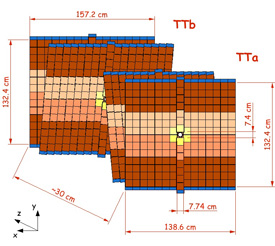
\includegraphics[width=0.49\linewidth]{figures/TT-layout.jpg}
   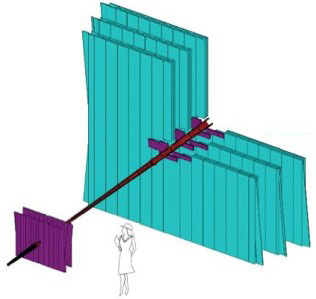
\includegraphics[width=0.49\linewidth]{figures/Tracking-system-diagram-2.jpg}
   \caption{Layout of the TT station (left) and the schematic view of the whole ST system, the cartoon of the woman is shown to indicate the size of each detectors (right). Figure taken from \cite{lhcb}.  
     \label{fig:TT}}
 \end{center}
\end{figure}


One of the quantity that can be used to determine ST performance is the hit efficiency, which can be expressed as a ratio between the number of measured hits to the number of hits expected in a given region. This ratio was evaluated to be $99.7\%$ for TT and $99.8\%$ for the IT. This evaluation was performed on the data collected during Run 1. Another important metric to determine ST performance is the hit spatial resolution.  For 2012 the hit resolution was measured to be $53.4 \mu m$ for the TT and $54.9 \mu m$ for IT.  


\subsubsection{Outer Tracker}

 The Outer Tracker is a complementary element to the IT, designed to cover the remaining LHCb acceptance region and it is placed in tracking stations T1, T2, and T3.  Each of the OT modules is made of drift-time tubes filled with a gas mixture of $70\%$ of Argon and $30\%$ of $CO_2$. 
The Drift-time detector reconstructs the hit position by measuring the drift time of the ionization electron to the anode located at the center of the tube. The distance between the wire and the particle’s trajectory is determined by comparing the drift time with bunch crossing signals.  The ionization electron is created when a charged particle interacts with a gas. 
OT achieves drift time less than $50 ns$ which allows reconstructing hits with a spatial resolution of $200 \mu m$.   
OT has a consistent layout of the IT detector, which means it also has four modules in  $(X, U, V, X)$ orientation, which is shown in figure \ref{fig:OT}. 


\begin{figure}[h]
\centering
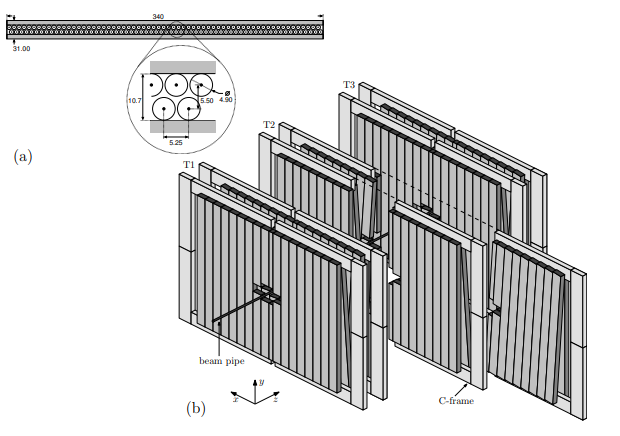
\includegraphics[scale=0.8]{figures/OT.PNG}
\caption{OT stations. Figure (a) presents the cross section of single OT module, all distances in $mm$, and the arrangement of OT modules in layers and stations around the beam pipe (b).  
\label{fig:OT}}
\end{figure}

\subsubsection{Magnet}

The LHCb Magnet plays a crucial role within the experiment, it bends the trajectory of the charged particle allowing to estimate its momentum. LHCb detector was equipped with a single warm dipole magnet. The Magnet is situated between TT and T tracking stations. 
Figure \ref{fig:magnet} shows a photography of the Magnet. It is composed of two identical saddle-shaped coils. These coils are placed inside an iron yoke, which was designed to be compatible with the acceptance of the LHCB detector. The coils are made of pure AI-99.7 with a 25 mm diameter central channel for water cooling. 

The estimated momentum resolution depends on the proper measurement of the magnetic field. Therefore, the diligent procedure to determine the shape of the magnetic field was as a function of the direction along the beam pipe, was conducted. As the outcome, the precision of the measurement of the magnetic field is quoted to be $4 \cdot 10 \%{-4} \delta B /B $ and the magnitude is 14 T, which is shown in figure \ref{fig:magnet}. 

To minimize the systematic reconstruction errors, which can play a dominant role in the precise measurement of $CP$ asymmetries,  the magnet operates in two polarities (positive and negative curves in figure \ref{fig:magnet}). The amount of data collected is approximately equal for both polarities and this split can be used to cross-check systematic reconstruction effects.   



\begin{figure}[h]
 \begin{center}
  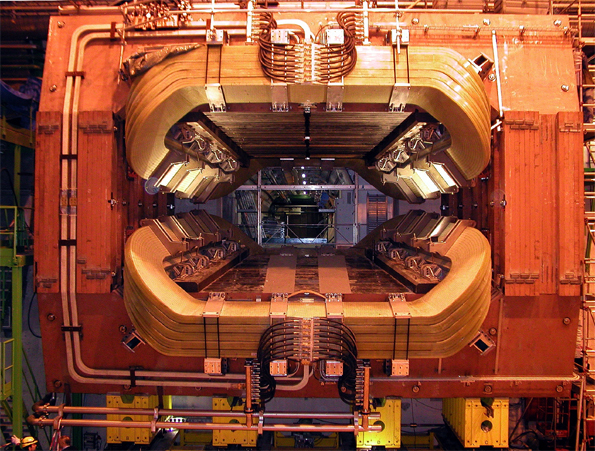
\includegraphics[width=0.49\linewidth]{figures/magnet_photo.jpg}
   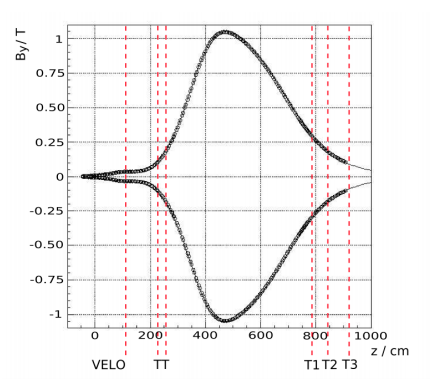
\includegraphics[width=0.49\linewidth]{figures/magnet_profile.PNG}
   \caption{The left is a photo of the LHCb Magnet taken after completion in 2004. The picture was taken towards the direction of the Velo detector, before other sub-detector have been installed, the visible part are coils (yellowish) and yoke (reddish). Magnetic field profile as a function of the $z$ axis (direction along the beam pipe). The red dashed lines corresponds to the location of the tracking sub-detectors (right). Figure taken from \cite{lhcb}.   
     \label{fig:magnet}}
 \end{center}
\end{figure}


\subsection{Particle identification}

Particle identification (PID) is an indispensable step to obtain any interesting physics results. For instance, the ability to significantly reduce the background often relies on the correct separation of kaons from pions.
The LHCb PID system is composed of two ring-imaging Cherenkov detectors (RICH), a series of muon chambers and a calorimeter system (ECAL and HCAL), see figure \ref{fig:LHCBlayout}. 

The combined information from these sub-detectors allows distinguishing between various types of charged particles. The problem consists of identifying the charged particle type associated with a given track. There are five relevant particle species, namely, electron, muon, pion, kaon, proton, and ghost track (charged tracks that do not correspond to a real particle which passed through the detector) making a total of six hypotheses. Therefore, this is a multiclass classification problem. 

The classical approach to this classification problem is to compute Log Likelihoods separately for each hypothesis and combining them: 
\begin{equation}
\Delta log \mathcal{L}_{A,B} = log \mathcal{L}_{A} - log \mathcal{L}_{A}  
\end{equation}
Where: $ \mathcal{L}_{A}$ and $ \mathcal{L}_{B}$ represents likelihood that a particle is identified under $A$ and $B$ hypothesis ( $A, B  \in \{ \pi, K, p, \mu, e \})$. The classification is performed by simply comparing the $DLL_{A,B}$ to a specific threshold. When the $DLL_{A,B}$ is greater than the threshold, it means that the particle is likely to be $A$. 

The enhancement to the ordinary negative log likelihood is application of the multivariate analysis. The model that was proposed and deployed is a fully-connected neural network (that kind of model is described in section \ref{sec:DNN}) with one hidden-layer implemented using the TMVA package \cite{TMVA}. The model is called ProbNN. These baseline models proved that the application of Machine Learning could significantly improve the performance of Particle identification. The figure \ref{fig:PID baseline} shows performance comparisons, measured as a ROC curve \footnote{for a formal definition of ROC curve see section \ref{sec:ROC}} between these two models.

\begin{figure}[h]
 \begin{center}
  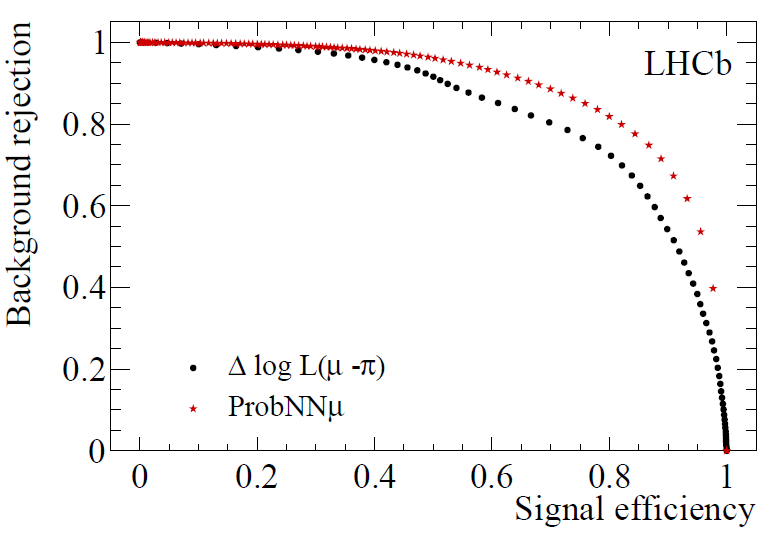
\includegraphics[width=0.49\linewidth]{figures/PID_prob_left.PNG}
   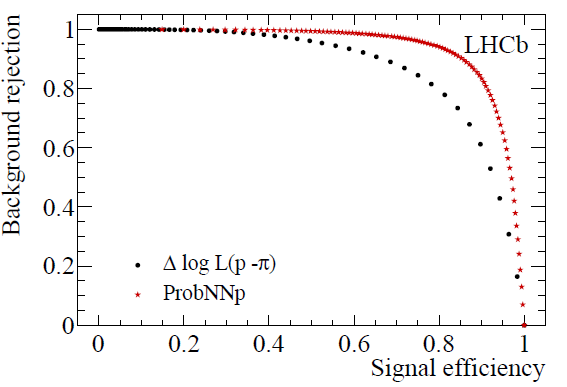
\includegraphics[width=0.49\linewidth]{figures/PID_prob_right.PNG}
    \caption{Background misidentification rates versus muon (left) and proton (right)
identification efficiency. The variables $\Delta \mathcal{L} (X −\pi)$
(black) and ProbNN (red), are compared for 5 − 10 $GeV\/c$ muons and 5 − 50 $GeV\/c$ protons,
using data sidebands for backgrounds and simulated samples for the signal. The data sample
used corresponds to 2012 sample collected at center-of-mass energy 8 GeV.}%
\label{fig:PID baseline}%
 \end{center}
\end{figure}

The overall Particle Identification performance can be summarize by the following numbers:

\begin{itemize}
    \item Electrons: $90\%$ identification efficiency with about $5\%$ electron to hadron missidentification probability. 
    \item Kaons: identification efficiency averaged over the momentum range of\\ $2-100~ GeV/c$ is $95\%$ with a nearly $5\%$ pion to kaon missidentification rate. 
    \item Muon: $97\%$ identification efficiency with pion to muon missidentification rate in between $1$ and $3\%$.  
\end{itemize}


The remainder of this section is dedicated to present each of the components of the Particle Identification system.


\subsubsection{RICH detector}

The most important component of the Particle Identification system is the Ring Imaging Cherenkov detector (RICH). LHCb has two of these detectors installed. The first one, called RICH1, is placed just before TT and the second one (RICH2) after T stations, see \ref{fig:LHCBlayout}. These detectors were designed to identify charged particles over a large momentum range of $2-100~ GeV/c$. To accomplish this task RICH1 was filled $C_4F_{10}$ gas radiator, which allows covering a momentum range from $2-100~ GeV/c$, which corresponds to the low-momentum particles, including those that are swept out of the detector acceptance. In contrast, RICH2 is filled with $CF_4$, which can be used to cover the momentum range of  $15-100~ GeV/c$. The geometry of both RICH1 and RICH2 detectors are presented in figures \ref{fig:RICH1} and \ref{fig:RICH2} respectively. 


\begin{figure}[h]
 \begin{center}
  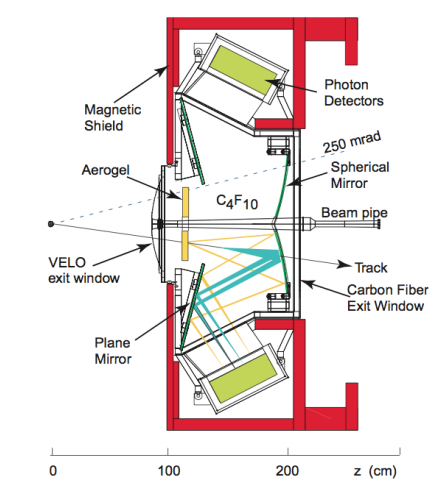
\includegraphics[width=0.49\linewidth]{figures/RICH1.PNG}
   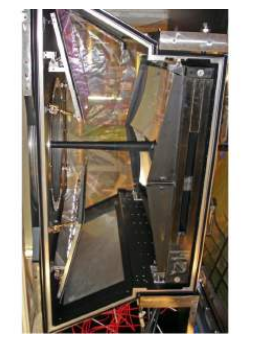
\includegraphics[width=0.49\linewidth]{figures/RICH1_photo.PNG}
    \caption{Geometry of the low momentum RICH detector (left), photo of the RICH1 detector (right). Figures taken from \cite{lhcb}}%
\label{fig:RICH1}%
 \end{center}
\end{figure}


\begin{figure}[h]
 \begin{center}
  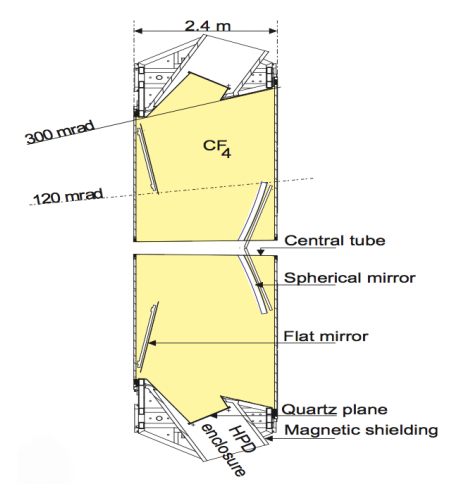
\includegraphics[width=0.49\linewidth]{figures/RICH2.PNG}
   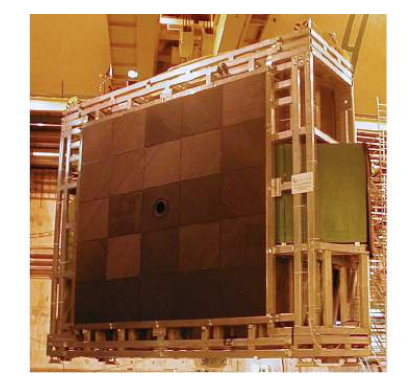
\includegraphics[width=0.49\linewidth]{figures/RICH2_photo.PNG}
    \caption{Geometry of the high momentum RICH detector (left), photo of the RICH2 detector (right). Figures taken from \cite{lhcb}}%
    \label{fig:RICH2}%
 \end{center}
\end{figure}


The RICH detector works by measuring Cherenkov radiation emitted when the charged particle traverse through the detector. Cherenkov radiation is emitted when a charged particle moves through a medium at the velocity higher than the speed of light at this medium. The emitted radiation angle ($\theta_c$) depends directly on the particle velocity and it is expressed by:

\begin{equation}
cos \theta_c = \frac{1}{n\beta}
\end{equation}

Where: $\beta$ is the velocity of the particle divided by the speed of light, and $n = \frac{c}{v_{medium}}$. 

Once emitted, Cherenkov radiation is reflected via a combination of spherical and flat mirrors to hybrid photon detectors (HPD). The HPD has a photocathode that emits electron when excited by the Cherenkov radiation. This electron is accelerated by a potential of about 20kV toward a silicon detector, which allows identifying the location of the hit. The performance, understood as a identification efficiency, of the RICH detector is shown in figure \ref{fig:RICH_performance}. 


\begin{figure}[h]
 \begin{center}
  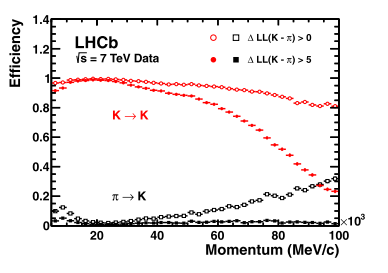
\includegraphics[width=0.49\linewidth]{figures/Kaon_proton.PNG}
   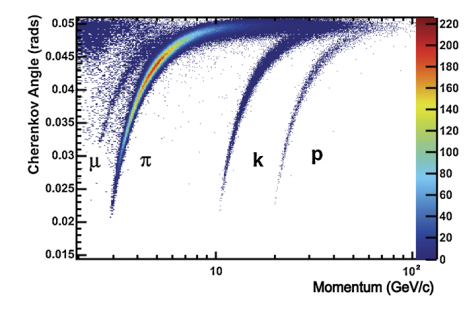
\includegraphics[width=0.49\linewidth]{figures/Chernkov_angle.PNG}
    \caption{Kaon identification efficiency and pion misidentification rate measured using simulated events as a function of track momentum. Two different $\Delta log \mathcal{L}(K − \pi)$ requirements have been imposed on the
samples (left), reconstructed Cherenkov angle as a function of track momentum in the $C_4F_{10}$ radiator (right). Figures taken from \cite{RICH_performance}}%
    \label{fig:RICH_performance}%
 \end{center}
\end{figure}


\subsubsection{Muon Stations}

The proper muon identification is an essential requirement because muons are the final decay states of some of the most important heavy flavor decays such as $B_s^0 \rightarrow J/\psi ~~ \mu^{+}\mu^{-}$,  $B^{0}_s \rightarrow K^{*0} ~~ \mu^{+}\mu^{-}$ and they can be used as an initial flavor tag for measurements of $B^0$  and $B^0_{s}$ oscillations. 

The muon system provides muon identification as a Log-Likelihood which depends on the track momentum and the number of hits detected in muon stations and how close the hits are with respect to the extrapolated track position in the muon system. It also provides such information as $x,y$ position in the muon station, which can be used for standalone-track reconstruction, and $p_T$ information which is used by the L0 trigger system, for a more details refer to section \ref{sec:trigger}. Therefore, the muon station is read out at the frequency of $40 Mhz$. 

Muon stations are located the farthest from the interaction point. The placement of these detectors is dictated by the fact that muons don’t interact strongly, have a high masses ($105~ MeV/c^2$), and long lifetime ($2.2 \cdot 10^{-6}s$) thus muons travels much farther than any other charged particles.  
  
The muon system is composed of five stations, one situated just before the calorimeter and four downstream from the calorimeter. Each of the stations is composed of two types of detectors. The first one is a multiwire proportional chamber located far from the beam pipe and triple gas electron multiplier (GEM) detectors \footnote{GEM detector is used due to the higher particle flux} placed in central quadrants close to the beam. Those detector use gas mixture consisting of $Ar$, $CO_2$ and $CF_4$. A cartoon of the muon station is shown in figure \ref{fig:muon}. 
The efficiency of the muon identification is, on average, above $98\%$ with pion and kaon misidentification rate below $1\%$, which is shown in figure \ref{fig:muon_missidentify}. 


\begin{figure}[h]
 \begin{center}
  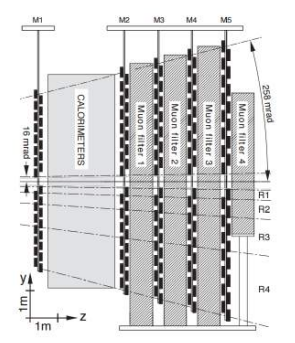
\includegraphics[width=0.49\linewidth]{figures/muon_stations.PNG}
   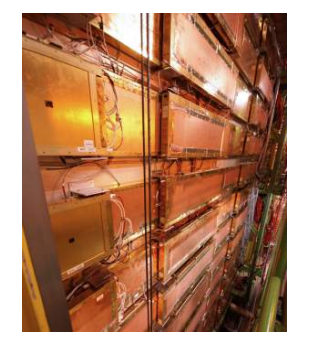
\includegraphics[width=0.49\linewidth]{figures/muon_photo.PNG}
    \caption{Site view of the muon detector (left) and a photo of M5 station. Figures taken from \cite{lhcb}.}%
    \label{fig:RICH_performance}%
 \end{center}
\end{figure}



\begin{figure}[h]
\centering
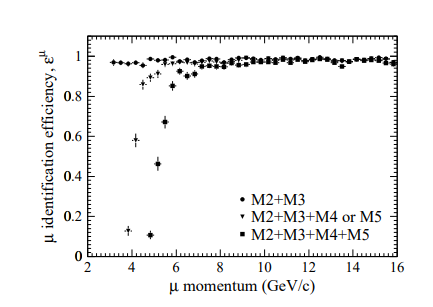
\includegraphics[scale=0.6]{figures/muon_eff.PNG}
\caption{Muon-identification efficiency as a function of momentum, for different requirements on the number of hits. Figure taken from \cite{muon_tdr}.
\label{fig:muon_missidentify}}
\end{figure}



\subsubsection{Calorimeters}

The calorimeter system performs several functions. It is responsible for providing fast information for the hardware trigger level and allows identification of electrons, photons, and hadrons, jointly with a measurement of their energies and transverse positions.

The calorimeter system is designed to measure the energy of an interacting particle. This is achieved via measuring the energy of a secondary electromagnetic and/or hadronic shower which is created when the particle travels through an absorber material. This measurement is performed by scintillators or silicon detectors. The measured energy is the total energy of all showers absorbed in the active materials, thus corresponds to the initial energy of the initial particle. 

The calorimeter system consists of an Electromagnetic calorimeter (ECAL) and Hadron Calorimeter.  Both are placed between the first and second muon stations, see \ref{fig:LHCBlayout}. ECAL subdetector is dedicated to identifying photons and electrons.  It is equipped with two additional detectors, placed in front of it, a PreShower detector (PS) and a Scintillator Pad Detector (SPD), the layout and granularity of both are presented in figure \ref{fig:ECAL}. 


PS and the SPD are used by the low-level trigger to distinguish electrons from photons and pions. The information about the number of tracks per event obtained by SPD is also used by the trigger to disregard those events that are too crowded. 
The ECAL is made of 2 mm lead plates followed by a 4 mm scintillator pad (shashlik like layout).  Its granularity depends on the distance from the beam, see figure \ref{fig:ECAL}.
The energy resolution of the ECAL detector can be expressed: 

\begin{equation}
    \frac{\sigma_{E}}{E} = \frac{10\%}{\sqrt{E/GeV}} \oplus	 1 \%
\end{equation}
where: $\oplus $ denote addition in quadrature which can be formulated as: 
\begin{equation}
   \Delta a\oplus \Delta b = \sqrt{\Delta a^2 + \Delta b^2} 
\end{equation}


\begin{figure}
\centering
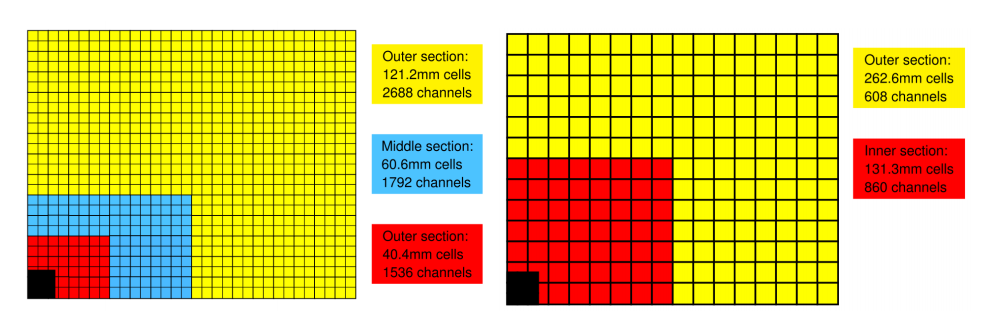
\includegraphics[width=\linewidth]{figures/ECAL.PNG}
\caption{Granularity for the different detector regions of the SPD, PS, and ECAL (left)
and of the HCAL (right). Figure taken from \cite{lhcb}.
\label{fig:ECAL}}
\end{figure}

The HCAL has a alternating structure of iron and scintillator tiles. The scintillator tiles are 4 mm tick and the iron ones are 16 mm. The HCAL energy resolution, obtained from the testbeam data are expressed: 

\begin{equation}
    \frac{\sigma_E}{E} = \frac{(69\pm 5) \%}{\sqrt{E}} \oplus (9\pm 2) \%
\end{equation}
 
\section{LHCb trigger}

LHCb trigger system was designed to make a fast decision, the trigger is a real-time application, whether or not to keep the data readout by the detectors. Its goal is to select heavy flavor decays from other proton-proton interactions. The trigger was implemented to reduce the data rate from the initial bunch crossing rate of 40 MHz to about 5kHz of data recorded on tapes. The initial data rate is several orders of magnitude above the current abilities of data recording and storage, and the events that are interesting form the physics point of view and would be taken for further studies compose of a tiny fraction of the overall rate of proton-proton collisions.  The data rate reduction is achieved by making a fast decision based on approximate measurement of particle transverse momentum and energy, muon identification, track displacement, and topological properties which allows discriminating some specific decays. 

The trigger system is composed of two sub-systems. The first one, called Level-0 trigger (L0), is completely implemented in hardware through the use of FPGA’s \footnote{FPGA stands from Field Programmable Gate Arrays, which are a semiconducting device based on a matrix of configurable logic blocks connected via programable interconnection. Their design has a benefit with respect to a CPU that allows massive parallelism since FPGA programable blocks can work independently and simultaneously. } L0 trigger usees the information from calorimeters and muon detector to reduce the bunch-crossing rate to below 1.1 MHz, which is the maximum input rate fo the front-end ASICs used in Velo and ST.  It is divided into three independend trigger decisions (L0 pileup, L0 muon,L0 calorimeters) each of them has its own specific selections and the final decision is a combination of each through a logic “or”. 

The L0 pileup triggers contributes to luminosity measurements \cite{trigger}.
The L0 calorimeter trigger leverage the information from ECAL, the HCAL, the PS and the SPD. Its desision is mostly based on a transverse energy deposited in a cluster of $2\times 2$ cells of the same size. The transvers energy, which is rather odd units since the energy is a scalar not a vector, is defined as :

\begin{equation}
    E_T = \sum_{i=1}^{4} E_i \sin\theta_i
\end{equation}

Where $E_i$ is the energy deposited in cell $i$ and $\theta_i$ is the angle between the beam axis and the direction of the particle. 
This quantity is combined with information on the number of hits in the PS and SPD to distinguish between hadron, photon and electron candidates. 


Events accepted by the L0 trigger are sent to the Event Filter Farm, a computing cluster located at the LHCb pit, consisting of 29 000 cores during Run I and more than 50 000 cores during Run II.  This computing farm is responsible for running High Level Trigger (HLT) applications. Those applications were written in C++ and consist of a several trigger selections designed to collect specific events, for instance $b$ or $c$ hadron decays. The trigger strategy has changed over the course of years when LHCb detector collected the data. Figure \ref{fig:trigger} presents the triggering scheme for both Run I and Run II. 


\begin{figure}
\centering
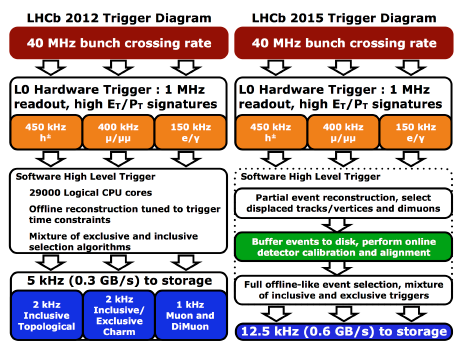
\includegraphics[width=\linewidth]{figures/trigger.PNG}
\caption{LHCb trigger flow during Run I (left) and Run II (right). Each graph illustrate a trigger selections and typical event acceptance rate after each stage. Figure taken from \cite{trigger_schame}.
\label{fig:trigger}}
\end{figure}

HLT consists of two stages, the first one called HLT1 evaluates a simplified version of tracking and muon reconstruction in order to quickly identify the track that could trigger an event. HLT 1 allows reducing the data flow going from the L0 trigger giving a sufficient amount of time to HLT2 to perform the more sophisticated reconstruction.

Within the HLT1 tracks are reconstructed in Velo and selected based on the probability that particular tracks originate from heavy flavor decays, which is achieved by determining their impact parameter. Selected tracks are then associated with track segments in the tracking stations, which allows estimation of the transverse momentum of the corresponding charged particle. This information together with track’s $\chi^2$ and impact parameter $\chi^2_{IP}$ is used to select interesting events.  
During Run II, a small portion of data selected by HLT1 is used to calibration and alignment of the detectors. This process, which takes a few minutes, is performed to reduce the probability of misalignment on the tracker. Any misalignment would impact the momentum resolution affecting the quality of reconstruction in HLT2. 

The HLT2 constitute of two types of algorithm inclusive and exclusive ones. Exclusive algorithms are used to select specific decays at the trigger level. For instance, they required all decay products to be reconstructed. 
Inclusive trigger selections, also called topological lines, trigger on partially-reconstructed $b$ hadrons decays. Those lines are designed to collect all $b$ hadrons decays with a displaced secondary vertex and at least two charged particles in the final state.
The quality of reconstruction in the HLT2 during Run II allowed LHCb to implement so-called “Turbo” lines that return fully reconstructed analysis-ready data. Additionally, those lines allow saving space by discarding the raw data, keeping only the relevant information describing reconstructed events. 

The trigger efficiency is estimated using TITOS method, described in great detail in \cite{trigger_eff}. 

What is worth to notice, the algorithm described in chapter \ref{chapter ML algo} was executed as a part of the HLT2. 

\section{LHCb software}

In order to generate Monte Carlo simulated samples (see figure \ref{fig:lhcb_sim}) and analyze data collected by the detectors, the LHCb collaboration designed and implemented a number of packages \cite{lhcb_software}. Most of them were implemented in  C++ and they are based on two frameworks ROOT \cite{root} and Gaudi \cite{gaudi}. The list below contains a brief description of selected packages:

\begin{itemize}
    \item \textbf{Gauss} \cite{gauss} was designed to generate the initial particles and simulates their transport through the LHCb detector. The Gauss application consists of two major independent processing phases. The first one is a generation of the primary events whose outcome is particles coming out of the primary proton-proton collision. This generation is handled by the PYTHIA \cite{pythia} a general-purpose event generator, whist the decay and time evolution of the produced particles is delegated to EventGen \cite{eventGen}. The second phase of Gauss application: detector response simulation is performed via customized Geant4 \cite{geant4} based module. 
    \item \textbf{Bool} performs a final stage of the LHCb detector simulation. It applies the detector response to hits previously generated by the Gauss. This step, called digitization, includes simulation of the detector and read-out electronics response, together with  L0 trigger hardware information. The Bool’s output format mimics the data coming from the real detector.
    \item \textbf{Brunel} this package is responsible for the whole process of data reconstruction, which consist of retrieving all recorded hits in a detector, doing the pattern recognition to identify trajectories, finding primary vertices of interaction and assigning PID likelihood. Brunel can process both simulated and the real collected by detector data. The outcome of the Brunel are reconstructed object (e.g tracks described in chapter \ref{chapter ML algo}) are saved in a Data Summary Tape (DST) files.   
    \item  \textbf{DaVinci} was designed to process the Brunel output and based on it reconstruct decays of interest and apply selection criteria to reduce the background. The outcome of this step is a dataset containing decay candidates for the user-specific decay topologies, which are used as a starting point for further physics analysis.   
    
\end{itemize}


\begin{figure}[!h]
\centering
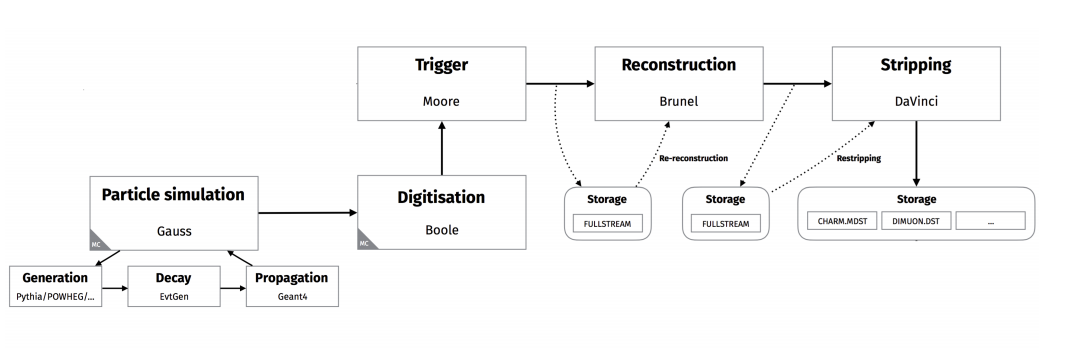
\includegraphics[width=\linewidth]{figures/LHCb_simulation.PNG}
\caption{LHCb event simulation flow. Each rectangle with a sharp corners represents a separated LHCb package described in text. Figure taken from  \cite{lhcb_computing}.
\label{fig:lhcb_sim}}
\end{figure}



\section{LHCb upgrade}
This section is divided into three parts. The first one is dedicated to presents the general concept of why LHCb collaboration decided to upgrade its detector. The second one describes the scope of the Upgrade by discussing which elements will be replaced. The final subsection focuses on the Upstream Tracker detector. It provides a very detailed description of this detector since the author was personally involved in its development.  

\subsection{Motivation}

The data collected during both Run I and Run II allowed to perform and report a number of precise measurements of rare decays of $b$ and $c$ hadrons, which were used to set new limits on models describing New Physics. Although, some of the precise measurements are still limited by statistical uncertainties and continuing data collection at the current rate wouldn’t allow to decrease them to the expected by theory level. In order to increase annual data yields, the LHCb detector must undergo a major upgrade during the Long Shutdown II.  The changs will allow the detector to operate at the increased luminosity level to $20 \times 10^{33} cm^{-2}s^{-1}$, which is five times higher than the current one. The new detector is expected to read data at the bunch crossing rate of 40 MHz, which allows collecting about $5~ fb^{-1}$ per year while during both Run I and Run II LHCb collected nearly $8~ fb^{-1}$. Figure \ref{fig:lhcb_lumi} present the luminosity plan. This figure also presents prediction of the longer term future of the LHCb experiment, which is out of scope of this thesis.  

\begin{figure}[!h]
\centering
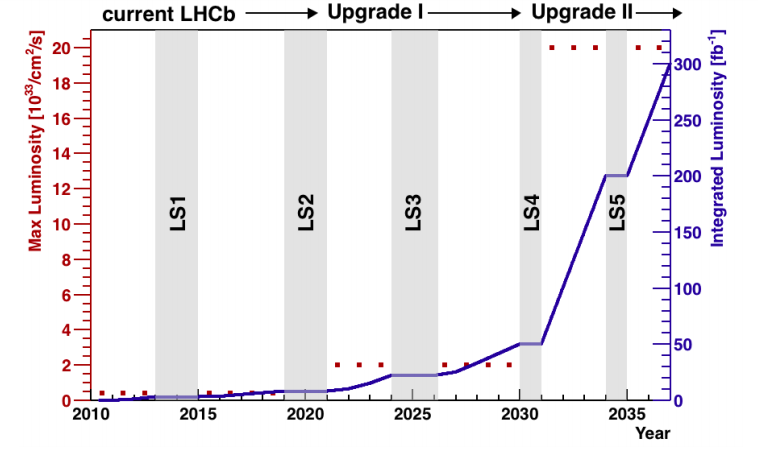
\includegraphics[width=\linewidth]{figures/lhcb_lumi.PNG}
\caption{Luminosity plan from 2010 to 2037 for the LHCb experiment. Red dots represent
the value of measured or predicted instantaneous luminosity. Solid blue line represents the value of measured or predicted integrated luminosity.
\label{fig:lhcb_lumi}}
\end{figure}


\subsection{General aspects of the LHCb Upgrade}

One of the main limitations that drive the idea of the LHCb Upgrade is the collision rate, which must be reduced to 1.1 MHz. This limitation comes from the specific of the current readout system, see section \ref{sec:velo}.  To overcome this limitation all tracking detector and their readout system has to be replaced to be capable of reading out the full detectors at $40 ~MHz$ rate. New read-out electronic will allow removing the L0 trigger, keeping only the software flexible part. Figure \ref{lhcb_upgrade} presents the new layout of the LHCb detector. When comparing this layout with the current one, see figure \ref{fig:LHCBlayout}, it is clearly visible that the entire structure of the detector stays as it was, only tracking detectors will be replaced. In fact, the detectors that currently are used by the L0 trigger will not have major interventions. 

\begin{figure}[!h]
\centering
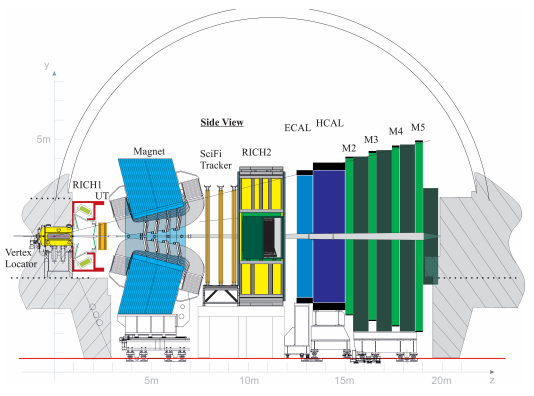
\includegraphics[width=\linewidth]{figures/LHCb_upgrade.PNG}
\caption{Layout of the upgraded LHCb detector. Figure taken from \cite{upgrade_tdr}
\label{fig:LHCBlayout}}
\end{figure}

\subsection{Upgraded Velo}
The upgraded Velo detector, which is the only upgraded tracking detector that keeps its old name, will be placed closer to the beam, its active area starting at the distance of $5.1 mm$ from the beam axis and it will have a finer granularity. The new Velo will operate at the higher particle flux going through it due to increased luminosity which causes an increase in the average number of visible proton-proton collisions from 1.7 to 5.2. To reduce occupancy on the readout channels, the microstrips were replaced by pixels. The upgraded Velo detector will consist of 41 million $55\times 55 \mu m$ pixels, which will be read-out by the custom-build VeloPix front-end ASIC, at the 40 MHz rates. 
The cooling is provided by evaporative CO2 circulating within miniature channels embedded in the modules.
A layout of the upgraded Velo module is shown in figure \ref{fig:veloUpgradeModule}. 
The expected improvement of the impact parameter reconstruction efficiency is shown in figure \ref{fig:upgrade_velo_performance}.    

\begin{figure}[!h]
\centering
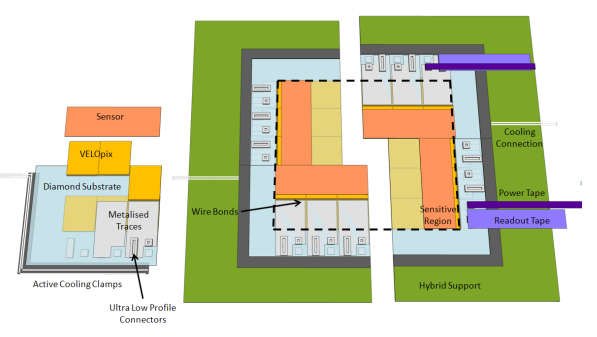
\includegraphics[width=\linewidth]{figures/Velo_upgraded_module.PNG}
\caption{Layout of a module of the upgraded VELO detector. Figure taken from \cite{velo_upgrade_tdr}
\label{fig:veloUpgradeModule}}
\end{figure}




\begin{figure}[!h]
 \begin{center}
  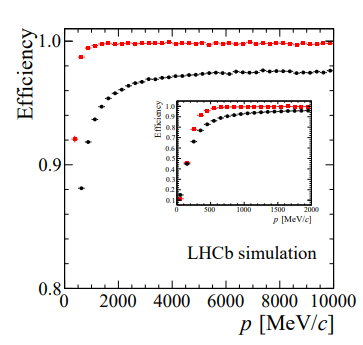
\includegraphics[width=0.49\linewidth]{figures/Velo_upgrade_tracking.PNG}
   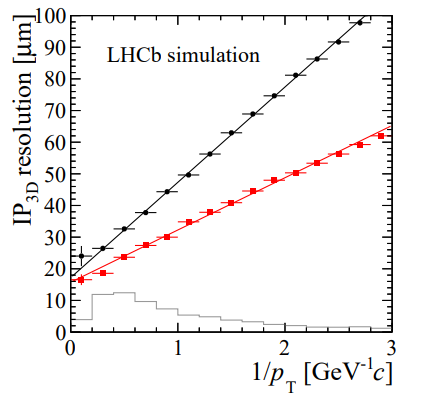
\includegraphics[width=0.49\linewidth]{figures/Velo_upgrade_IP.PNG}
    \caption{The left figure shows the reconstruction efficiency for particles which are reconstructible as Velo tracks as a function of momentum. The right plot shows the  3D resolution of the IP, the light gray histogram shows the relative population of $b$ hadron daughter tracks in each $1/p_t$ bin. Figures taken from \cite{velo_upgrade_tdr}.}%
    \label{fig:upgrade_velo_performance}%
 \end{center}
\end{figure}

\subsection{Scintillating Fibre Tracker}

Scintillating Fibre Tracker (SciFi) was designed to replace the T stations. This decision was driven by two factors. Extensive simulations studies showed that the upgraded condition would be too harsh for OT, the foreseen occupancy would be too high to provide reliable input to the tracking pattern recognition algorithm. Moreover, the readout electronics of both OT and IT detectors would not be capable of working as a part of a new data acquisition system. SciFi covers the full detector acceptance downstream to the magnet and, by design, guarantees a spatial resolution of nearly $80 \mu m$. 
This detector will consist of three stations, each of them composed of four detection planes organized, similar to IT,  in a $(X, U, V, X)$ orientation, see figure \ref{fig:SciFI}.
 The module will consist of scintillating fibres with a radius of  $125 \mu m$. and a length of 2.5 m, which will be read out by Silicon PhotoMultipliers (SiPMs), located either at the top and bottom of the detector. The SiPMs are kept in a cold box, at $-40 \circ C$, to reduce the dark count rate \footnote{The dark count rate, is the count rate that is measured in the absence of photons, is caused by thermally generated electron-hole pairs.} and each of them consist of nearly 100 pixels.   


\begin{figure}[!h]
\centering
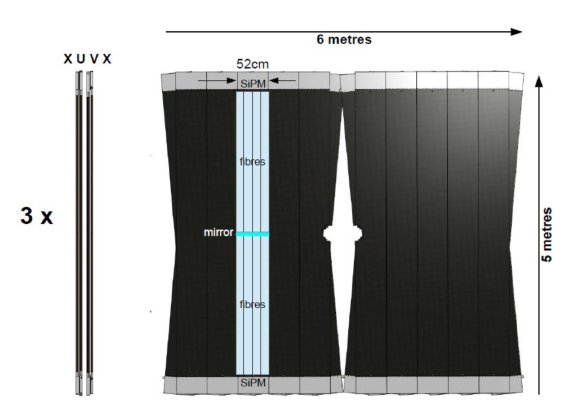
\includegraphics[scale=0.6]{figures/SciFi.PNG}
\caption{Layout of one tracking station of the SciFi detector. Figure taken from \cite{upgrade_tracker_tdr}
\label{fig:SciFI}}
\end{figure}

The SciFi detection mechanism is based on measuring the photons emitted when a particle traverses the detector’s active area. Those photons are propagated through the fibres and finally reach the pixels located at the end of the fibres. A signal  proportional to the number of fired pixels within a given SiPM channel is used to determinate the position of the particle, which is shown in figure \ref{fig:SciFI_idea}. 


\begin{figure}[!h]
\centering
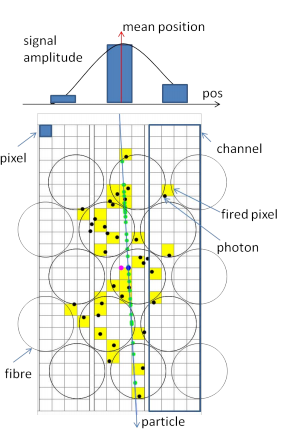
\includegraphics[scale=0.5]{figures/SciFi_idea.PNG}
\caption{Visualization of the detection mechanism of the SciFi. The squares shows the pixel located at the fibers end and the circles indicate the cross-section of the scintillating fibres. Note that, the fibres are not aligned to the detector channels and the photons can arrive at the detector outside the fibre area.  Figure taken from \cite{upgrade_tracker_tdr}
\label{fig:SciFI_idea}}
\end{figure}

 